\documentclass{beamer}
\usepackage[english, russian]{babel}
\usepackage[T2A]{fontenc}
\usepackage[utf8]{inputenc}
\usepackage{indentfirst}
\usepackage{amsmath, amsfonts, amssymb, amsthm, mathtools}
\usepackage[export]{adjustbox}
\usepackage{graphicx} 
\graphicspath{ {./images/} }

\usepackage{subcaption}
\usepackage{verbatim}

\usepackage{minted}{\setlength{\parskip}{0pt}}

\usepackage{hyperref}

\hypersetup{
    colorlinks=true,
    linkcolor=blue,
    filecolor=magenta,      
    urlcolor=black,
    pdftitle={Overleaf Example},
    pdfpagemode=FullScreen,
    }


\title{Отчет по лабораторной работе № 7. \\ Расширенные настройки межсетевого экрана}
\author{Данила Стариков \\ НПИбд-02-22}
\date{2024}

\begin{document}

\maketitle
\newpage

\tableofcontents

\newpage
\section{Цель работы}
Получить навыки настройки межсетевого экрана в Linux в части переадресации
портов и настройки Masquerading.
\newpage

\section{Выполнение работы}
\subsection{Создание пользовательской службы firewalld}
\begin{enumerate}
\item Загрузили операционную систему и перешли в рабочий каталог с проектом:
    \begin{minted}{bash}
cd ~/tmp/dastarikov/vagrant/
    \end{minted}
\item Запустили виртуальную машину server:
    \begin{minted}{bash}
make server-up
    \end{minted}
\item На виртуальной машине server вошли под своимk пользователем и открыли терминал. Перешли в режим суперпользователя:
    \begin{minted}{bash}
sudo -i
    \end{minted}
\item На основе существующего файла описания службы ssh создали файл с собственным описанием:
    \begin{minted}{bash}
cp /usr/lib/firewalld/services/ssh.xml /etc/firewalld/services/ssh-custom.xml
cd /etc/firewalld/services/
    \end{minted}
\item Посмотрели содержимое файла службы (Рис. \ref{img:0}):
    \begin{minted}{bash}
cat /etc/firewalld/services/ssh-custom.xml
    \end{minted}

\begin{center}
    \centering
    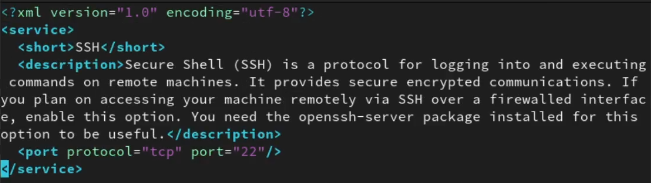
\includegraphics[width=\textwidth]{../images/image00.png}
    \captionof{figure}{Содержимое файла ssh.xml по умолчанию}
    \label{img:0}
\end{center}

\item Открыли файл описания службы на редактирование и заменили порт 22 на новый
порт (2022):
    \begin{minted}{xml}
<port protocol="tcp" port="2022"/>
    \end{minted}
    Скорректировали описание службы, чтобы отметить, что она была изменена.
\item Просмотрели список доступных FirewallD служб (Рис. \ref{img:1}):
    \begin{minted}{bash}
firewall-cmd --get-services
    \end{minted}

\begin{center}
    \centering
    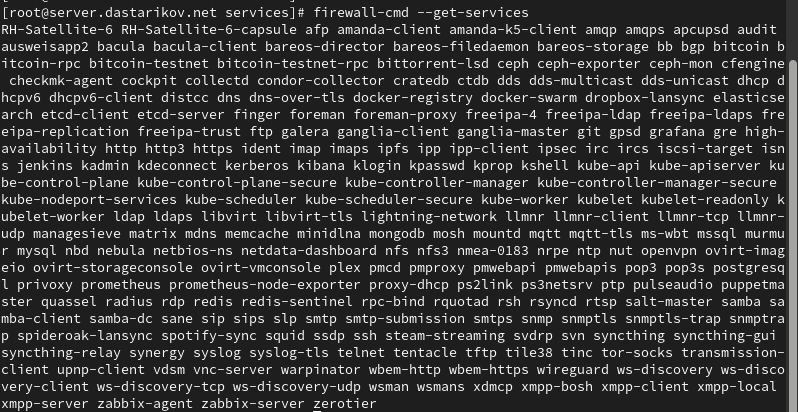
\includegraphics[width=\textwidth]{../images/image01.png}
    \captionof{figure}{Список доступных служб.}
    \label{img:1}
\end{center}

Новая служба ещё не отображается в списке.
\item Перегрузили правила межсетевого экрана с сохранением информации о состоянии и вновь вывели на экран список служб, а также список активных служб (Рис. \ref{img:2}):
    \begin{minted}{bash}
firewall-cmd --reload
firewall-cmd --get-services
firewall-cmd --list-services
    \end{minted}

\begin{center}
    \centering
    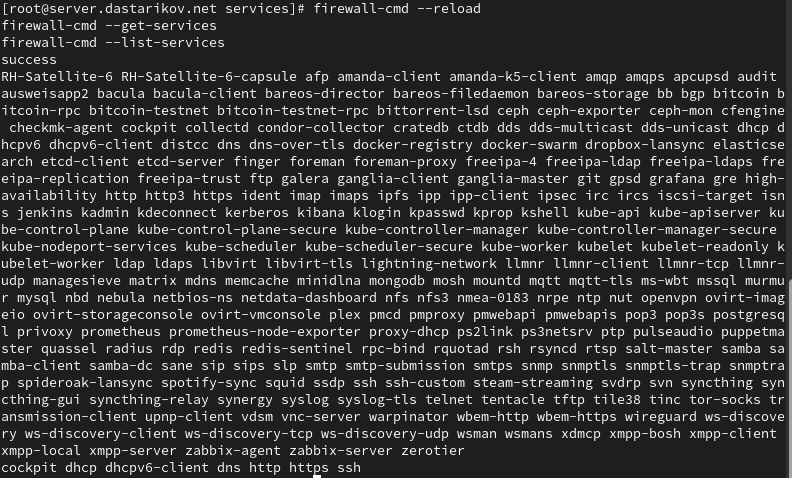
\includegraphics[width=\textwidth]{../images/image02.png}
    \captionof{figure}{Список доступных и активных служб после обновления.}
    \label{img:2}
\end{center}

    Созданная служба ssh-custom отобразилась в списке доступных для FirewallD служб, но не активирована.
\item Добавили новую службу в FirewallD и вывели на экран список активных служб (Рис. \ref{img:3}):
    \begin{minted}{bash}
firewall-cmd --add-service=ssh-custom
firewall-cmd --list-services
    \end{minted}

\begin{center}
    \centering
    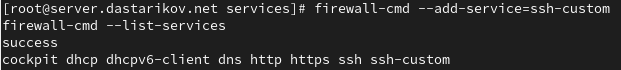
\includegraphics[width=\textwidth]{../images/image03.png}
    \captionof{figure}{Список активных слухб после добавления ssh-custom.}
    \label{img:3}
\end{center}

\item Служба была успешно добавлена в список активных, далее перегрузили правила межсетевого экрана с сохранением информации о состоянии (Рис. \ref{img:4}):
    \begin{minted}{bash}
firewall-cmd --add-service=ssh-custom --permanent
firewall-cmd --reload
    \end{minted}

\begin{center}
    \centering
    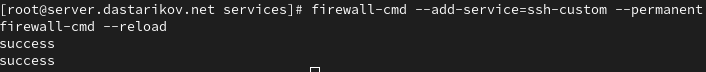
\includegraphics[width=\textwidth]{../images/image04.png}
    \captionof{figure}{Сохранение информации о состоянии и перезагрузка службы firewalld.}
    \label{img:4}
\end{center}

\end{enumerate}

\subsection{Перенаправление портов}
\begin{enumerate}
\item Организовали на сервере переадресацию с порта 2022 на порт 22 (Рис. \ref{img:5}):
    \begin{minted}{bash}
firewall-cmd --add-forward-port=port=2022:proto=tcp:toport=22
    \end{minted}

\begin{center}
    \centering
    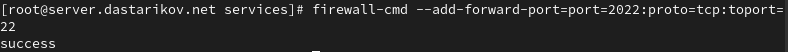
\includegraphics[width=\textwidth]{../images/image05.png}
    \captionof{figure}{Успешное добавление переадресации с порта 2022 на порт 22.}
    \label{img:5}
\end{center}

\item На клиенте попробовали получить доступ по SSH к серверу через порт 2022 (Рис. \ref{img:6}):
    \begin{minted}{bash}
ssh -p 2022 dastarikov@server.dastarikov.net
    \end{minted}

\begin{center}
    \centering
    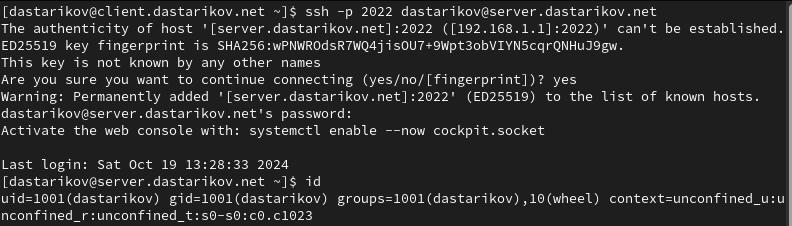
\includegraphics[width=\textwidth]{../images/image06.png}
    \captionof{figure}{Получение доступа по SSH на клиенте.}
    \label{img:6}
\end{center}

\end{enumerate}

\subsection{Настройка Port Forwarding и Masquerading}
\begin{enumerate}
    \item На сервере посмотрели, активирована ли в ядре системы возможность перенаправления IPv4\-пакетов пакетов (Рис. \ref{img:7}):
    \begin{minted}{bash}
sysctl -a | grep forward
    \end{minted}

\begin{center}
    \centering
    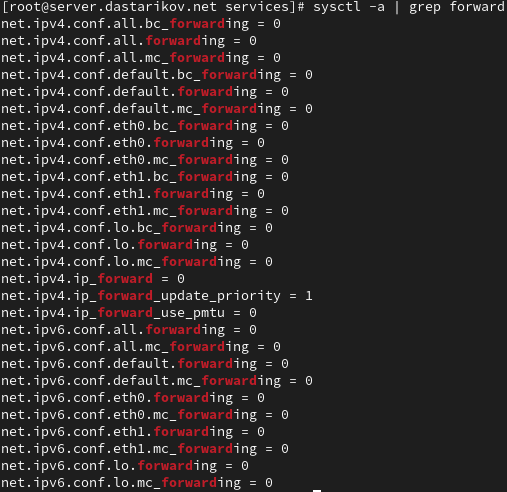
\includegraphics[width=\textwidth]{../images/image07.png}
    \captionof{figure}{Список параметров, связанных с перенарпавлением пакетов.}
    \label{img:7}
\end{center}

\item Включили перенаправление IPv4\-пакетов на сервере (Рис. \ref{img:9}):
    \begin{minted}{bash}
echo "net.ipv4.ip_forward = 1" > /etc/sysctl.d/90-forward.conf
sysctl -p /etc/sysctl.d/90-forward.conf
    \end{minted}

\begin{center}
    \centering
    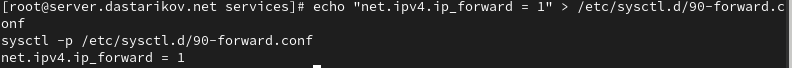
\includegraphics[width=\textwidth]{../images/image09.png}
    \captionof{figure}{Включение перенапрвления IPv4\-пакетов на сервере.}
    \label{img:9}
\end{center}

\item Включили маскарадинг на сервере (Рис. \ref{img:10}):
    \begin{minted}{bash}
firewall-cmd --zone=public --add-masquerade --permanent
firewall-cmd --reload
    \end{minted}

\begin{center}
    \centering
    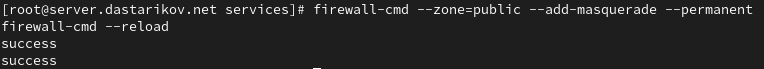
\includegraphics[width=\textwidth]{../images/image10.png}
    \captionof{figure}{Включение маскарадинга на сервере.}
    \label{img:10}
\end{center}

\item На клиенте проверили доступность выхода в Интернет (Рис. \ref{img:11}).

\begin{center}
    \centering
    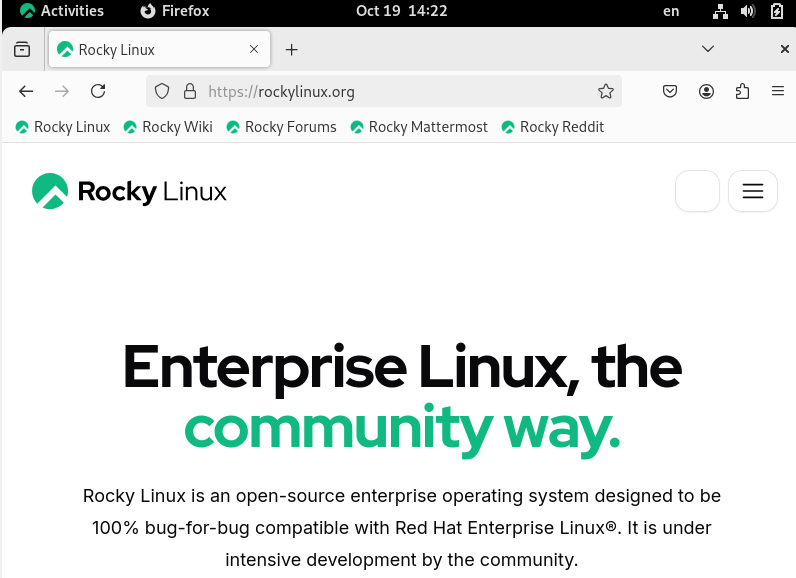
\includegraphics[width=\textwidth]{../images/image11.png}
    \captionof{figure}{Проверка доступности Интернета на клиенте.}
    \label{img:11}
\end{center}

\end{enumerate}

\subsection{Внесение изменений в настройки внутреннего окружения виртуальной машины}
\begin{enumerate}
\item На виртуальной машине server перешли в каталог для внесения изменений
в настройки внутреннего окружения /vagrant/provision/server/, создайте в нём
каталог firewall, в который поместили в соответствующие подкаталоги конфигура-
ционные файлы FirewallD (Рис. \ref{img:12}):
    \begin{minted}{bash}
cd /vagrant/provision/server
mkdir -p /vagrant/provision/server/firewall/etc/firewalld/services
mkdir -p /vagrant/provision/server/firewall/etc/sysctl.d
cp -r /etc/firewalld/services/ssh-custom.xml /vagrant/provision/server/firewall/etc/firewalld/services/
cp -r /etc/sysctl.d/90-forward.conf /vagrant/provision/server/firewall/etc/sysctl.d/
    \end{minted}
\item В каталоге /vagrant/provision/server создали файл firewall.sh (Рис. \ref{img:12}):
    \begin{minted}{bash}
cd /vagrant/provision/server
touch firewall.sh
chmod +x firewall.sh
    \end{minted}

\begin{center}
    \centering
    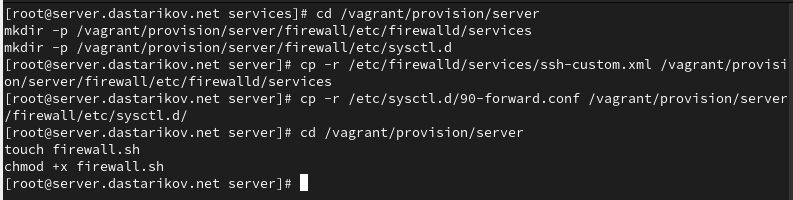
\includegraphics[width=\textwidth]{../images/image12.png}
    \captionof{figure}{Создание каталога с конфигурацией firewalld.}
    \label{img:12}
\end{center}

    Прописал в нем следующий скрипт:
    \begin{minted}{bash}
#!/bin/shell
echo "Provisioning script \$0"
echo "Copy configuration files"
cp -R /vagrant/provision/server/firewall/etc/* /etc
echo "Configure masquerading"
firewall-cmd --add-service=ssh-custom --permanent
firewall-cmd --add-forward-port=port=2022:proto=tcp:toport=22 --permanent
firewall-cmd --zone=public --add-masquerade --permanent
firewall-cmd --reload
restorecon -vR /etc
    \end{minted}
\item Для отработки созданного скрипта во время загрузки виртуальной машины server в конфигурационном файле Vagrantfile добавили в разделе конфигурации для сервера (Рис. \ref{img:13}):
    \begin{minted}{bash}
server.vm.provision "server firewall",
type: "shell",
preserve_order: true,
path: "provision/server/firewall.sh"
    \end{minted}

\begin{center}
    \centering
    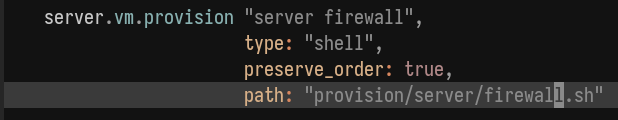
\includegraphics[width=\textwidth]{../images/image13.png}
    \captionof{figure}{Изменение Vagrantfile.}
    \label{img:13}
\end{center}

\end{enumerate}

\section{Ответы на контрольные вопросы}
\begin{enumerate}
\item Где хранятся пользовательские файлы firewalld?

    Файлы хранятся в каталоге /etc/firewalld/.
\item Какую строку надо включить в пользовательский файл службы, чтобы указать порт TCP 2022?

    Строку \texttt{<port protocol="tcp" port="2022"/>}.
\item Какая команда позволяет вам перечислить все службы, доступные в настоящее время на вашем сервере?

    \texttt{firewall-cmd --get-services}.
\item В чем разница между трансляцией сетевых адресов (NAT) и маскарадингом (masquerading)?

    При трансляции сетевого адреса локальный IP-адрес преобразуется во внешний адрес, в то время как при маскарадинге локальный адрес заменяется на адрес связывающей машины.
\item Какая команда разрешает входящий трафик на порт 4404 и перенаправляет его в службу ssh по IP-адресу 10.0.0.10?

    \texttt{firewall-cmd --add-forward-port=port=4404:proto=tcp:toaddr=10.0.0.10:toport=22}
\item Какая команда используется для включения маcкарадинга IP-пакетов для всех пакетов, выходящих в зону public?

    \texttt{firewall-cmd --zone=public --add-masquerade}
\end{enumerate}

\newpage
\section{Выводы}
В результате выполнения лабораторной работы продолжили изучать настройки межсетевого экрана в Linux, настроили переадресацию портов и Masquerading.

\end{document}
